\documentclass{beamer}

\mode<presentation>{
\usetheme{Warsaw} %{Berkeley}
% \usecolortheme{dolphin}
\setbeamercovered{transparent} 
\setbeamertemplate{navigation symbols}{}
}

% Definições latex para portugues
\usepackage[utf8]{inputenc}
\usepackage[brazil]{babel}
\usepackage[T1]{fontenc}

% Formatação de URL
\usepackage{url}

% Adição de figuras no documento
\usepackage{graphicx}
\usepackage{setspace}
\usepackage{graphics}

% Definições matemáticas
\usepackage{amsmath}
\usepackage{amsfonts}

% Tabelas longas (mais de uma página)
\usepackage{longtable}
\usepackage{rotating}
\usepackage{array}
\usepackage{multirow}

% definicoes
\newtheorem{teo}{Teorema}
\newtheorem{defin}{Definição}

%  ABACO -- Conjunto de macros para desenhar o 'abaco

%  Desenho original de Hans Liesenberg

%  Macros de Tomasz Kowaltowski

%  DCC -- IMECC -- UNICAMP

%  Mar,co de 1988  --  Vers~ao 1.0

% Ajustado para LaTeX da SUN -- Mar,co de 1991

% ---------------------------------------------------------

%  Chamada:   \ABACO{d1}{d2}{d3}{d4}{esc}
%             com:  di's -- os quatro d'igitos;
%	           esc  -- fator de escala

% ---------------------------------------------------------

%  DEFINI,C~OES AUXILIARES

% ---------------------------------------------------------


%  Forma o d'igito pequeno (0 ou 1)

\newcommand{\ABACODP}[1]{%
%
\thicklines
%    
\begin{picture}(8,0)
    \ifcase#1{   %  caso 0
       \put(0,0)    {\line(1,0){4}}
       \multiput(5,0)(2,0){2}{\oval(2,4)}}
    \or{         %  caso 1
       \put(2,0)    {\line(1,0){4}}
       \multiput(1,0)(6,0){2}{\oval(2,4)}}
    \fi
\end{picture}
    } % \ABACODP

% Forma o d'igito grande (0 a 4)

\newcommand{\ABACODG}[1]{%
%
\thicklines
%    
\begin{picture}(14,0)
    \ifcase#1{   % caso 0
       \multiput(1,0)(2,0){5}{\oval(2,4)}}
       \put(10,0)   {\line(1,0){4}}
    \or{         % caso 1
       \multiput(1,0)(2,0){4}{\oval(2,4)}}
       \put(8,0)   {\line(1,0){4}}
       \put(13,0)   {\oval(2,4)}
    \or{         % caso 2
       \multiput(1,0)(2,0){3}{\oval(2,4)}
       \put(6,0)   {\line(1,0){4}}
       \multiput(11,0)(2,0){2}{\oval(2,4)}}
    \or{         % caso 3
       \multiput(1,0)(2,0){2}{\oval(2,4)}
       \put(4,0)   {\line(1,0){4}}
       \multiput(9,0)(2,0){3}{\oval(2,4)}}
    \or{         % caso 4
       \put(1,0)  {\oval(2,4)}}
       \put(2,0)   {\line(1,0){4}}
       \multiput(7,0)(2,0){4}{\oval(2,4)}
    \fi
\end{picture}
    } % \ABACODG
       
% Forma um d'igito (0 a 9)

\newcommand{\ABACOD}[1]{%
%
    \ifnum#1>9
       \errmessage{#1: Argumento invalido para ABACO}
    \fi
    \ifnum#1<0
       \errmessage{#1: Argumento invalido para ABACO}
    \fi
%
\begin{picture}(24,0)
%    
    \ifnum#1<5
       \put(16,0) {\ABACODP{0}}
    \else   
       \put(16,0) {\ABACODP{1}}
    \fi
%    
    \ifnum#1<5
       \put(0,0)  {\ABACODG{#1}}
    \else
       \ifcase#1\or \or \or \or
          \or  \put(0,0)  {\ABACODG{0}}
          \or  \put(0,0)  {\ABACODG{1}}
          \or  \put(0,0)  {\ABACODG{2}}
          \or  \put(0,0)  {\ABACODG{3}}
          \or  \put(0,0)  {\ABACODG{4}}
       \fi
    \fi   
\end{picture}
    } % \ABACOD
    
% -------------------------------------------------

%  DEFINI,C~AO PRINCIPAL
    
\newcommand{\ABACO}[5]{%
    \setlength{\unitlength}{#5mm}
%
    \thinlines
%   
\begin{picture}(28,25)
%   
% moldura
%
% externa
%
        \put(0,0)            {\line(0,1){25}}
        \put(0,0)            {\line(1,0){28}}
        \put(28,0)           {\line(0,1){25}}
        \put(0,25)           {\line(1,0){28}}
% interna
        \put(2,2)            {\line(0,1){21}}
	\put(26,2)           {\line(0,1){21}}
	\put(16,2)           {\line(0,1){21}}
	\put(18,2)           {\line(0,1){21}}
	\put(2,2)            {\line(1,0){14}}
	\put(16,2)           {\line(1,-1){1}}
	\put(17,1)           {\line(1,1){1}}
	\put(18,2)           {\line(1,0){8}}
	\put(2,23)           {\line(1,0){14}}
	\put(16,23)          {\line(1,1){1}}
	\put(17,24)          {\line(1,-1){1}}
	\put(18,23)          {\line(1,0){8}}
	\put(0,0)            {\line(1,1){2}}
	\put(0,25)           {\line(1,-1){2}}
	\put(28,0)           {\line(-1,1){2}}
	\put(28,25)          {\line(-1,-1){2}}
%
%   
% d'igitos
%
%   
       \put(2,20)  {\ABACOD{#1}}
       \put(2,15)  {\ABACOD{#2}}
       \put(2,10)  {\ABACOD{#3}}
       \put(2,5)   {\ABACOD{#4}}
%      
\end{picture}
    } % \ABACO
    


\title[CP aplicada a Problemas de Rearranjo de Genomas]{Programação por
Restrições aplicada a Problemas de Rearranjo de Genomas}

\author{Victor de Abreu Iizuka\\ Orientador: Zanoni Dias}

\institute[UNICAMP]{\textbf{Instituto de Computação,Univesidade Estadual
de Campinas}\\ \begin{columns}[t]
    \begin{column}{5cm}
        \vspace{-1.2cm}
        \begin{figure}
            \centering
            
\includegraphics[scale=0.4]{images/unicamp-logo.jpg}
        \end{figure} 
    \end{column}
    \begin{column}{5cm} 
        \parbox{1in}{\center{\ABACO{2}{0}{1}{2}{0.7}}}
    \end{column}
\end{columns}}

\date{}

\begin{document}

\frame{\titlepage}

\frame{\tableofcontents}

\section{Introdução}

\frame{\frametitle{Introdução [1/4]}

\begin{itemize} 

    \item{Rearranjo de genomas tem como o objetivo encontrar o menor
        número de operações que transformam um genoma em outro.}

    \item{Essas operações podem ser reversões, transposições, fissões e
        fusões.}

    \item{Estudos mostram que rearranjos são mais adequados que mutações
        pontuais quando se deseja comparar os genomas de duas espécies
        [Palmer and Herbon (1988), Bafna and Pevzner~(1995)].}

\end{itemize}}

\frame{\frametitle{Introdução [2/4]}

\begin{itemize} 
    
    \item{Neste contexto, a distância evolutiva é o menor número de
        operações que são necessárias para transformar um genoma em
        outro.}

    \item{Neste trabalho, trataremos os casos em que os eventos de
        reversões e transposições ocorrem de forma isolada e os casos
        quando os dois eventos ocorrem ao mesmo tempo.}

\end{itemize}}

\frame{\frametitle{Introdução [3/4]}

\begin{itemize}

    \item{O trabalho desenvolvido nesta dissertação segue a linha de
        pesquisa utilizada por Dias e Dias~(2009) e nós apresentaremos
        modelos de Programação por Restrições (CP) para ordenação por
        reversões e ordenação por reversões e transposições, baseados na
        teoria do Problema de Satisfação de Restrições (CSP) e na teoria
        do Problema de Otimização com Restrições (COP).}

\end{itemize}}

\frame{\frametitle{Introdução [4/4]}

\begin{itemize}

    \item{Nós fizemos comparações com os modelos de Programação por
        Restrições para ordenação por transposições, descrito por Dias e
        Dias~(2009), e no caso de ordenação por reversões e ordenação
        por reversões e transposições, com os modelos de Programação
        Linear Inteira (ILP) descritos por Dias e Souza~(2007).}

\end{itemize}}
%%% \end{Introdução} %%%

\frame{\frametitle{Permutação}

\begin{itemize}

    \item{Para fins computacionais, um genoma é representado por uma
        $n$-tupla de genes, e quando não há genes repetidos essa tupla é
        chamada de permutação.}

    \item{Uma permutação é representada como $\pi =
        (\pi_{1}~\pi_{2}~\ldots~\pi_{n})$, para $\pi_{i} \in
        \mathbb{N}$, $0 < \pi_{i} \leq n$ e $i \neq j \leftrightarrow
        \pi_{i} \neq \pi_{j}$.}

    \item{A permutação identidade é representada como $\iota =
        (1~2~3~\ldots~n)$.}
    
\end{itemize}} 

\subsection{Problema da Distância de Reversão} 

\frame{\frametitle{Problema da Distância de Reversão [1/3]} 

\begin{beamerboxesrounded}[center,shadow=true]{Evento de reversão:} 
    \footnotesize
    Um evento de reversão ocorre quando um bloco do genoma é invertido.
    \normalsize
\end{beamerboxesrounded} 

\begin{columns}[t] 
    \begin{column}{5cm} 
        \begin{figure}
            \centering 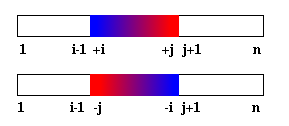
\includegraphics[width=4.5cm]{images/rev02.png}
            \caption{Uma reversão aplicada sobre uma permutação
            orientada.}
        \end{figure} 
    \end{column}
    \begin{column}{5cm} 
        \begin{figure} 
            \centering
            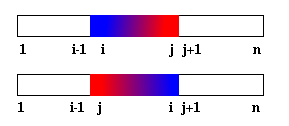
\includegraphics[width=4.5cm]{images/rev01.png} 
            \caption{Uma reversão aplicada sobre uma permutação não
            orientada.} 
        \end{figure} 
    \end{column}
\end{columns} }

\frame{\frametitle{Problema da Distância de Reversão [2/3]} 

\begin{itemize} 
    
    \item{O Problema da Distância de Reversão é encontrar o número
        mínimo de reversões necessárias para transformar uma genoma em
        outro.}

    \item{O Problema da Distância de Reversão é equivalente ao problema de
        Ordenação por Reversões, que é a distância de reversão entre a
        permutação $\pi$ e a permutação identidade $\iota$, denotado por
        $d_{r}(\pi)$.}

\end{itemize}}

\frame{\frametitle{Problema da Distância de Reversão [3/3]} 

\begin{itemize} 
    
    \item{Se a orientação dos genes é conhecida, o problema pode ser
        solucionado com algoritmos polinomiais.}

    \item{Caso contrário, o problema pertence à classe de problemas
        NP-Difíceis, com a prova apresentada por Caprara (1997).}  

    \item{Melhor algoritmo de aproximação possui razão de $1.375$ e foi
        apresentado por by Berman, Hannenhalli and Karpinski (2002).}

\end{itemize} }

\frame{\frametitle{Grafo de Breakpoints para Reversões [1/4]} 

\begin{beamerboxesrounded}[center,shadow=true]{Breakpoints:}  
    \footnotesize
    Dois elementos consecutivos $\pi_{i}$ e $\pi_{i+1}$, $0 \le i \le
    n$, são \textit{adjacentes} quando $|\pi_{i} - \pi_{i+1}| = 1$, e
    são \textit{breakpoints} caso contrário. 
    \normalsize
\end{beamerboxesrounded}

\begin{itemize} 
    
    \item{A permutação $\pi$ é estendida adicionando os elementos
        $\pi_{0} = 0$ e $\pi_{n+1} = n+1$.}

    \item{Grafo de arestas coloridas $G(\pi)$ com $n+2$ vértices \{$0,
        1,~\ldots~, n, n+1$\}.}

    \item{Uma aresta preta liga os vértices $i$ e $j$ se $(i, j)$ for um
        \textit{breakpoint}.}

    \item{Uma aresta cinza liga os vértices $i$ e $j$ se $|i - j| = 1$ e
        os dois não são consecutivos em $\pi$.}

\end{itemize} }

\frame{\frametitle{Grafo de Breakpoints para Reversões [2/4]} 

\begin{columns}[t]
    \begin{column}{5cm}
        \begin{figure}
            \centering
            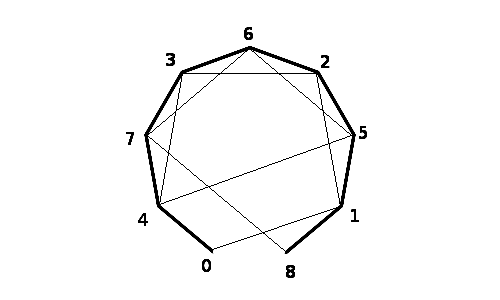
\includegraphics[width=5cm]{images/rev_grafo_bkp.png}
            \caption{Grafo de \textit{Breakpoints} da permutação $\pi =
        (4~7~3~6~2~5~1)$}
        \end{figure}
        \vspace{1cm}
    \end{column}
    \begin{column}{5cm}
        \begin{itemize}
            
            \footnotesize
            \item{Reversão atua em dois pontos em uma permutação,
                    portanto pode reduzir o número de breakpoints em
                    pelo menos um e no máximo dois.}
            \normalsize

        \end{itemize}
        
        \vspace{0.8cm}

        \begin{beamerboxesrounded}[center,shadow=true]{Teorema 1:}
            \footnotesize
            Para qualquer permutação $\pi$, 
            \[\frac{1}{2} b_r(\pi) \leq d_r(\pi) \leq
                b_r(\pi).
            \]
            \normalsize
        \end{beamerboxesrounded}
    \end{column}
\end{columns} }

\frame{\frametitle{Grafo de Breakpoints para Reversões [3/4]}

\begin{figure}[h]
    \centering 
    \begin{tabular}{ccc} 
        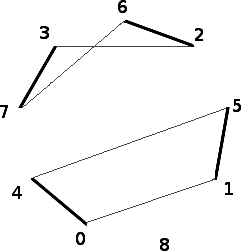
\includegraphics[scale=0.35]{images/rev_grafo_bkp_dec2cic-1.png}
        & ~~~~
        & 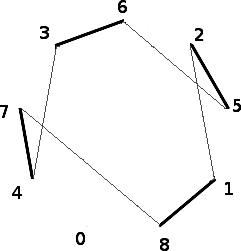
\includegraphics[scale=0.35]{images/rev_grafo_bkp_dec2cic-2.png} 
    \end{tabular} 
    \caption{Exemplo de decomposição em ciclos de arestas disjuntas para
        o grafo de \textit{breakpoints} da permutação $\pi =
    (4~7~3~6~2~5~1)$.}
\end{figure} }

\frame{\frametitle{Grafo de Breakpoints para Reversões [4/4]}

\begin{itemize}

    \item{O grafo pode ser decomposto em ciclos de arestas disjuntas.}

    \item{Existem diversas maneiras de realizar a decomposição.}

    \item{O Teorema 2, demonstrado no trabalho de Christie (1998),
          fornece os limitantes para a distância de reversão usando a
          quantidade de 2-ciclos na máxima decomposição de ciclos de
          $G(\pi)$.}

\end{itemize}

\vspace{0.5cm}

\begin{beamerboxesrounded}[center,shadow=true]{Teorema 2:}
    \footnotesize
    Se $c_{2}(\pi)$ é o número mínimo de $2$-ciclos em qualquer máxima
    decomposição em ciclos de $G(\pi)$ então: 
    \[
        \frac{2}{3} b_r(\pi)
        - \frac{1}{3} c_{2}(\pi) \leq d_r(\pi) \leq b_r(\pi) - \frac{1}{2}
        c_{2}(\pi).
    \]
    \normalsize
\end{beamerboxesrounded} }

\subsection{Problema da Distância de Transposição} 

\frame{\frametitle{Problema da Distância de Transposição [1/2]}

\begin{beamerboxesrounded}[center,shadow=true]{Evento de transposição:} 
    Um evento de transposição ocorre quando dois blocos adjacentes no
    genoma trocam de posição.
\end{beamerboxesrounded} 

\begin{figure} 
    \centering
    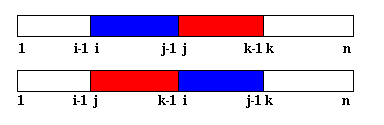
\includegraphics[width=6cm]{images/transv.png} 
    \caption{Uma transposição aplicada em uma permutação.}
\end{figure} }

\frame{\frametitle{Problema da Distância de Transposição [2/2]}

\begin{itemize}

    \item{O Problema da Distância de Transposição é encontrar o número
        mínimo de reversões necessárias para transformar um genoma em
        outro.} 

    \item{O Problema da Distância de Transposição é equivalente ao
            problema de Ordenação por Transposições, que é a distância
            de transposição entre a permutação $\pi$ e a permutação
            identidade $\iota$, denotado por $d_{t}(\pi)$.}

    \item{Pertence à classe de problemas NP-Difíceis, a prova foi
            apresentada por Bulteau, Fertin and Rusu (2010).} 

    \item{O melhor algoritmo de aproximação possui razão de $1.375$ e
            foi apresentado por Elias and Hartman (2006).} 

\end{itemize} }

\frame{\frametitle{Breakpoints para Transposições} 

\begin{beamerboxesrounded}[center,shadow=true]{Breakpoints:}  
    \footnotesize
    Um \textit{breakpoint} é um par $(\pi_{i}, \pi_{i+1})$, tal que
    $\pi_{i+1} \neq \pi_{i} + 1$. 
    \normalsize
\end{beamerboxesrounded}

\begin{itemize} 
    
    \item{A permutação $\pi$ é estendida adicionando os elementos
        $\pi_{0} = 0$ e $\pi_{n+1} = n+1$.}

    \item{Uma transposição atua em três pontos de uma permutação, logo
            pode reduzir o número de \textit{breakpoints} em pelo menos
            e no máximo três.}

\end{itemize} 

\begin{beamerboxesrounded}[center,shadow=true]{Teorema 3:}
    \footnotesize
    Para qualquer permutação $\pi$, 
    \[\frac{1}{3} b_t(\pi) \leq d_t(\pi) \leq
        b_t(\pi).
    \]
    \normalsize
\end{beamerboxesrounded} }

\frame{\frametitle{Grafo de Ciclos [1/3]}

\begin{itemize}

    \item{Introduzido por Bafna e Pevzner (1998).}

    \item{Grafo direcionado com arestas coloridas $G(\pi)$ com $n+2$
          vértices $\{0,~1,~\ldots,~n,~n+1\}$.}

    \item{Arestas cinzas são direcionadas de $i-1$ para $i$.}

    \item{Arestas pretas são direcionadas de $\pi_i$ para $\pi_{i-1}$.}

\end{itemize} 


\begin{figure}
    \centering
    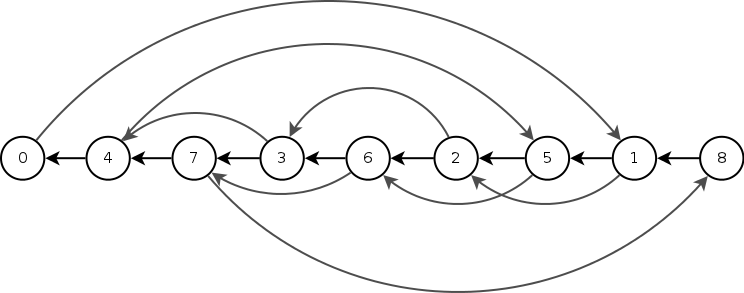
\includegraphics[width=8cm]{images/trans_cycle_graph.png}
    \caption{Grafo de ciclos da permutação $\pi = (4~7~3~6~2~5~1)$}
\end{figure} }


\frame{\frametitle{Grafo de Ciclos [2/3]}

\begin{figure}[h]
  \centering 
  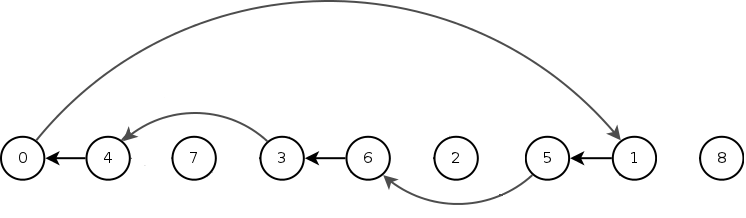
\includegraphics[width=8cm,height=2.4cm]{images/trans_cycle_graph_dec-1.png}
  \vspace{0.0001cm}
  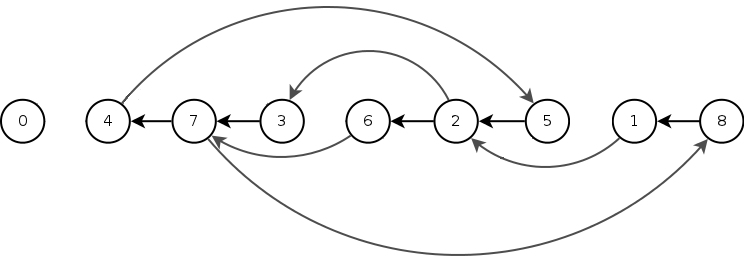
\includegraphics[width=8cm,height=2.8cm]{images/trans_cycle_graph_dec-2.png} 
  \caption{Exemplo de decomposição em ciclos de arestas disjuntas para
  o grafo de ciclos da permutação $\pi = (4~7~3~6~2~5~1)$.}
  \label{fig:tra_grafo_bkp_dec}
\end{figure} }


\frame{\frametitle{Grafo de Ciclos [3/3]}

\begin{itemize}

    \item{Para todo vértice de $G(\pi)$ toda aresta chegando é
        unicamente pareada com uma aresta saindo de cor diferente.}

    \item{Existe uma decomposição única de ciclos alternados do conjunto
        de arestas de $G(\pi)$.}

    \item{Seja $c_{\text{ímpar}}(\pi)$ o número de ciclos ímpares de
        $G(\pi)$, para uma permutação $\pi$, e $\Delta c_{\text{ímpar}}
        (\rho) = c_{\text{ímpar}} (\pi \rho) - c_{\text{ímpar}} (\pi)$ a
        mudança no número de ciclos ímpares devido a transposição
        $\rho$, temos que $\Delta c_{\text{ímpar}} \in \{2, 0, -2\}$,}

\end{itemize} 

\begin{beamerboxesrounded}[center,shadow=true]{Teorema 4:}
    \footnotesize
    Para qualquer permutação $\pi$, 
    \[ 
        \frac{1}{2}(n + 1 - c_{\text{ímpar}}(\pi)) \leq d_t(\pi) \leq
    \frac{3}{4} (n + 1 - c_{\text{ímpar}}(\pi)).  \]
    \normalsize
\end{beamerboxesrounded} }

\subsection{Problema da Distância de Reversão e Transposição} \frame{
\frametitle{Reversal and Transposition Distance Problem [1/1]} \begin{itemize}
    \item{The reversal and transposition distance problem is to find the
        minimum number of reversals and transpositions that transform one
        genome into another.} \item{Walter, Dias and Meidanis (1998, 2002) and
        Lin and Xue (1999) studied this problem.} \end{itemize} }

\section{Modelo} \frame{ \frametitle{Model [1/3]}
\begin{beamerboxesrounded}[center,shadow=true]{Permutation:} The permutation
    $\pi$ is a list of elements ($\pi_{1},\pi_{2},\cdots,\pi_{n}$) where
    $\pi_{i} \in \mathbb{N}$, $0 < \pi_{i} \le n$ and $\pi_{i} \neq \pi_{j}$
    for $i \neq j$. The identity permutation $\iota$ is defined as $\iota =
    (1~2~3~\cdots~n)$.  \end{beamerboxesrounded} \vspace{1cm} \scriptsize
    \begin{beamerboxesrounded}[center,shadow=true]{permutation/2}
        \vspace{-0.5cm} \begin{align} \textit{per}&\textit{mutation}(\pi,
            N)~\text{:-} \nonumber\\ &\textit{length}(\pi, N), \nonumber\\
            &\pi~::~[1~..~N], \nonumber\\ &\textit{all\_different}(\pi).
            \nonumber \end{align} \end{beamerboxesrounded} \normalsize }

\frame{ \frametitle{Model [2/3]}
\begin{beamerboxesrounded}[center,shadow=true]{Reversal:} A reversal
    $\rho(i,j)$, $0 < i < j \leq n$, split the list in three sub-lists
    $C_{1}C_{2}C_{3}$ where $C_{1} = (\pi_{1} .. \pi_{i-1})$, $C_{2} = (\pi_{i}
    .. \pi_{j})$ and $C_{3} = (\pi_{j+1} .. \pi_{n})$.  After that, we do a
    reverse on the sub-list $C_{2}$ and the result is the sub-list $R_{C_{2}}$.
    Finally we join the new sub-list $R_{C_{2}}$ with the sub-lists $C_{1}$ and
    $C_{3}$ to form $\rho\pi = C_{1}R_{C_{2}}C_{3}$.  \end{beamerboxesrounded}
    \vspace{0.1cm} \scriptsize
    \begin{beamerboxesrounded}[center,shadow=true]{reversal/4} \vspace{-0.5cm}
        \begin{align} \textit{rev}&\textit{ersal}(\pi, \sigma, I, J)~\text{:-}
            \nonumber\\ &\textit{permutation}(\pi, N), \nonumber\\
            &\textit{permutation}(\sigma, N), \nonumber \\ &1 \le I < J \le N,
            \nonumber\\ &\textit{split}(\pi, I, J, C_{1}, C_{2}, C_{3}),
            \nonumber\\ &\textit{reverse}(C_{2}, R_{C_{2}}), \nonumber \\
            &\sigma = C_{1}, R_{C_{2}}, C_{3}. \nonumber \end{align}
        \end{beamerboxesrounded} \normalsize }

\frame{ \frametitle{Model [3/3]}
\begin{beamerboxesrounded}[center,shadow=true]{Transposition:} A transposition
    $\rho(i,j,k)$, $0 < i < j < k\leq n$, split the list in four sub-lists
    $C_{1}C_{2}C_{3}C_{4}$ where $C_{1} = (\pi_{1} .. \pi_{i-1})$, $C_{2} =
    (\pi_{i} .. \pi_{j-1})$, $C_{3} = (\pi_{j} .. \pi_{k-1})$ and $C_{4} =
    (\pi_{k} .. \pi_{n})$. After we join them to form $\rho\pi =
    C_{1}C_{3}C_{2}C_{4}$. Note that $C_{1}$ and $C_{4}$ could be empty.
\end{beamerboxesrounded} \vspace{1cm} \scriptsize
\begin{beamerboxesrounded}[center,shadow=true]{transposition/5} \vspace{-0.5cm}
    \begin{align} \textit{tra}&\textit{nsposition}(\pi, \sigma, I, J,
        K)~\text{:-} \nonumber\\ &\textit{permutation}(\pi, N), \nonumber\\
        &\textit{permutation}(\sigma, N), \nonumber\\ &1 \le I < J < K \le N,
        \nonumber \\ &\textit{split}(\pi, I, J, K, C_{1}, C_{2}, C_{3}, C_{4}),
        \nonumber\\ &\sigma = C_{1}, C_{3}, C_{2}, C_{4}. \nonumber \end{align}
    \end{beamerboxesrounded} \normalsize }

\subsection{Modelo CSP} \frame{ \frametitle{CSP Model [1/3]} \begin{itemize}
    \item{We first model the problem as CSP.} \item{The number of variables is
        unknown because we need the value of distance $d_{r\_t}(\pi)$ to set
        the constraints and variables that represent the permutations.}
    \item{We pick a candidate value for distance $N$ such that $N \in [LB ..
        UB]$ and try to find the appropriate combination of $N$ reversals and
        transpositions.} \item{If the CSP fails, we choose another value for
        $N$ just incrementing its value.} \item{We check the value of $N$ using
        a bottom-up strategy.} \end{itemize} }

\frame{ \frametitle{CSP Model [2/3]} \scriptsize
\begin{beamerboxesrounded}[center,shadow=true]{rev\_trans\_dist/3}
    \vspace{-0.5cm} \begin{align} \textit{rev}&\textit{\_trans\_dist}(\iota, 0,
        \_Model). \nonumber\\ \textit{rev}&\textit{\_trans\_dist}(\pi, N,
        Model)~\text{:-} \nonumber\\ &\textit{bound}(\pi, Model, LB, UB),
        \nonumber\\ &N :: [LB .. UB], \nonumber\\ &\textit{indomain}(N),
        \nonumber \\ &\textit{event}(\pi, \sigma), \nonumber \\
        &\textit{rev\_trans\_dist}(\sigma, N-1, Model). \nonumber \end{align}
    \end{beamerboxesrounded} \normalsize }

\frame{ \frametitle{CSP Model [3/3]}
\begin{beamerboxesrounded}[center,shadow=true]{Bounds:} \begin{itemize}
    \item{\textbf{def\_csp} doesn't use any lower bounds.}
    \item{\textbf{r\_t\_br\_csp} chooses the best bound between the reversal
        breakpoint lower and upper bounds described by Bafna and Pevzner (1996)
        and the transposition breakpoint lower and upper bounds described by
        Bafna and Pevzner (1998).} \item{\textbf{r\_t\_bc\_csp} chooses the
        best bound between the reversal breakpoint lower and upper bounds and
        the transposition edge-colored cycle graph lower and upper bounds
        described by Bafna and Pevzner (1998).} \end{itemize}
    \end{beamerboxesrounded} }

\subsection{Modelo COP} \frame{ \frametitle{COP Model [1/5]} \begin{itemize}
    \item{Another approach is to model the problem as a COP.} \item{This
        approach needs an upper bound.} \item{We use the binary variables $B$
        to indicate whether an event, reversal or transposition, has modified
        the permutation.} \item{We use the same CSP bounds modified for COP
        models. So we have the following bounds: \textbf{def\_cop},
        \textbf{r\_t\_br\_cop} and \textbf{r\_t\_bc\_cop}.} \end{itemize} }

\frame{ \frametitle{COP Model [2/5]} \begin{itemize} \item{The first predicate
        that we need to create is \textit{reversal\_cop/5}. Given a permutation
        $\rho(i, j)$, we add a new clause to allow $(i, j) = (0, 0)$. If $(i,
        j) = (0, 0)$ then $\pi\rho = \pi$.} \item{The equivalent predicate for
        transposition is \textit{transposition\_cop/6}. Given a permutation
        $\rho(i, j, k)$, we add a new clause to allow $(i, j, k) = (0, 0, 0)$.
        If $(i, j, k) = (0, 0, 0)$ then $\pi\rho = \pi$.} \end{itemize}
        \begin{columns}[t] \begin{column}{5.5cm} \scriptsize
            \begin{beamerboxesrounded}[center,shadow=true]{reversal\_cop/5}
                \vspace{-0.5cm} \begin{align}
                    \textit{rev}&\textit{ersal\_cop}(\iota, \iota, 0, 0, 0).
                    \nonumber\\ \textit{rev}&\textit{ersal\_cop}(\pi, \sigma,
                    I, J, 1)~\text{:-} \nonumber\\ &\textit{reversal}(\pi,
                    \sigma, I, J). \nonumber \end{align}
                \end{beamerboxesrounded} \normalsize \end{column}
                \begin{column}{5.5cm} \scriptsize
                    \begin{beamerboxesrounded}[center,shadow=true]{transposition\_cop/6}
                        \vspace{-0.5cm} \begin{align}
                            \textit{tra}&\textit{nsposition\_cop}(\iota, \iota,
                            0, 0, 0, 0). \nonumber\\
                            \textit{tra}&\textit{nsposition\_cop}(\pi, \sigma,
                            I, J, K, 1)~\text{:-} \nonumber\\
                            &\textit{transposition}(\pi, \sigma, I, J, K).
                            \nonumber \end{align} \end{beamerboxesrounded}
                            \normalsize \end{column} \end{columns} }

\frame{ \frametitle{COP Model [3/5]} \begin{itemize} \item{To calculate the
        reversal and transposition distance in the COP model we implemented the
        \textit{rev\_trans\_dist\_cop/3} predicate.} \item{It sets the
        variables $B$ using the upper bound and constrains the permutations by
        making $\pi_{k} = \pi_{k-1} \rho_{k}$.} \item{\textit{length/2} is a
        prolog built-in and is used to create a list of non instantiated
        variables of a given size.} \item{The cost function \textit{Cost} is
        the sum of variables $B$ associated with each $\rho_{k}$, $Cost =
        \sum_{k=1}^{UB} B_{k}$.} \item{The reversal and transposition distance
        is the minimum value of the cost function $d_{r\_t} = \min Cost$.}
\end{itemize} }

\frame{ \frametitle{COP Model [4/5]} \scriptsize
\begin{beamerboxesrounded}[center,shadow=true]{rev\_trans\_dist\_cop/3}
    \vspace{-0.5cm} \begin{align} \textit{rev}&\textit{\_trans\_dist\_cop}(\pi,
        N, Model)~\text{:-} \nonumber\\ &\textit{bound}(\pi, Model, LB, UB),
        \nonumber\\ &\textit{length}(B, UB), \nonumber \\
        &\textit{upperbound\_constraint\_rev\_trans}(\pi, B, Model, UB),
        \nonumber\\ &\textit{sum}(B, Cost), \nonumber \\ &\textit{Cost} \ge
        \textit{LB}, \nonumber \\ &\textit{minimize}(Cost, N). \nonumber
    \end{align} \end{beamerboxesrounded} \normalsize }

\frame{ \frametitle{COP Model [5/5]}
\begin{beamerboxesrounded}[center,shadow=true]{the
    upperbound\_constraint\_rev\_trans:} The
    \textit{upperbound\_constraint\_rev\_trans/4} predicate applies the effects
    of $\rho_{k}$ in permutation and returns the value of $B$ for every
    reversal or transposition $\rho_{k}$.  \end{beamerboxesrounded}
    \vspace{1cm} \scriptsize
    \begin{beamerboxesrounded}[center,shadow=true]{upperbound\_constraint\_rev\_trans/4}
        \vspace{-0.5cm} \begin{align}
            \textit{upp}&\textit{erbound\_constraint\_rev\_trans}(\iota, [~],
            \_Model, \_UB). \nonumber\\
            \textit{upp}&\textit{erbound\_constraint\_rev\_trans}(\pi, [B|Bt],
            Model, UB)~\text{:-} \nonumber\\ &\textit{event\_cop}(\pi, \sigma,
            B), \nonumber\\ &\textit{bound}(\pi, Model, LB, \_UB), \nonumber\\
            &UB \ge LB, \nonumber \\
            &\textit{upperbound\_constraint\_rev\_trans}(\sigma, Bt, Model, UB
            - 1), \nonumber \end{align} \end{beamerboxesrounded} \normalsize }

\section{Análise dos Resultados} \frame{ \frametitle{Computational Experiments
[1/8]} \begin{itemize} \item{All the constraint logic programming models were
        implemented using: \begin{itemize} \item{Open source programming system
                \textit{ECLiPSe}.} \item{The proprietary C++ package
                \textit{IBM\textregistered{} ILOG\textregistered{}
                CPLEX\textregistered{} CP Optimizer}.} \end{itemize}} \item{All
                the integer programming formulations were implemented using:
                \begin{itemize} \item{Open source system \textit{GLPK}.}
                    \item{The proprietary C++ package
                        \textit{IBM\textregistered{} ILOG\textregistered{}
                        CPLEX\textregistered{} Optimizer}.} \end{itemize}}
                \end{itemize} }

\frame{ \frametitle{Computational Experiments [2/8]}
\begin{beamerboxesrounded}[center,shadow=true]{Computer Specifications:}
    \begin{itemize} \item{Intel\textregistered{}~Core\texttrademark~2 Duo
            2.33GHz.} \item{3 GB of RAM.} \item{Ubuntu Linux operating system
            with kernel 2.6.31.} \item{\textit{ECLiPSe-6.0}.}
        \item{\textit{GLPK-4.35}.} \item{\textit{IBM\textregistered{}
            ILOG\textregistered{} CPLEX\textregistered{} CP Optimizer v 2.3}.}
        \item{\textit{IBM\textregistered{} ILOG\textregistered{}
            CPLEX\textregistered{} Optimizer v 12.1}.} \end{itemize}
        \end{beamerboxesrounded} }

\frame{ \frametitle{Computational Experiments [3/8]} \begin{itemize} \item{The
        ILP results used the formulations described in Dias and Souza (2007).}
    \item{The column \textbf{size} represents the length of permutations used
        in the tests.} \item{The CPU times (in seconds) reported refers to an
        average of 50 instances where the permutation $\pi$ was randomly
        generated.} \item{We made a comparison between the permutation $\pi$
        and the identity permutation $\iota$.} \end{itemize} }

\frame{ \frametitle{Computational Experiments [4/8]} \tiny
\begin{center}
  \begin{tabular}{| r | r | r | r | r | r | r |} 
    \hline
    \multirow{2}{*}{\textbf{size}} & \multicolumn{6}{ c|}{\textbf{CP-ECLiPSe}} \\
    \cline{02-07}
    & \textbf{~def\_cop~} & \textbf{~r\_t\_br\_cop~} & \textbf{~r\_t\_bc\_cop~} & \textbf{~def\_csp~} & \textbf{~r\_t\_br\_csp~} & \textbf{~r\_t\_bc\_csp~} \\ 
    \hline
    ~3~  & ~0.034~ & ~0.012~  & ~0.003~   & ~0.004~   & ~0.003~    & ~0.002~ \\
    ~4~  & ~7.370~ & ~12.288~ & ~0.341~   & ~0.028~   & ~0.007~    & ~0.004~ \\ 
    ~5~  & ~-~     & ~-~      & ~26.047~  & ~0.343~   & ~0.020~    & ~0.010~ \\
    ~6~  & ~-~     & ~-~      & ~409.079~ & ~16.742~  & ~0.122~    & ~0.031~ \\
    ~7~  & ~-~     & ~-~      & ~-~       & ~593.666~ & ~0.670~    & ~0.104~ \\
    ~8~  & ~-~     & ~-~      & ~-~       & ~-~       & ~2.579~    & ~0.149~ \\
    ~9~  & ~-~     & ~-~      & ~-~       & ~-~       & ~13.958~   & ~0.339~ \\
    ~10~ & ~-~     & ~-~      & ~-~       & ~-~       & ~64.208~   & ~1.318~ \\
    ~11~ & ~-~     & ~-~      & ~-~       & ~-~       & ~167.423~  & ~3.327~ \\
    ~12~ & ~-~     & ~-~      & ~-~       & ~-~       & ~1058.050~ & ~11.044~ \\
    ~13~ & ~-~     & ~-~      & ~-~       & ~-~       & ~-~        & ~20.961~ \\
    ~14~ & ~-~     & ~-~      & ~-~       & ~-~       & ~-~        & ~51.294~ \\
    ~15~ & ~-~     & ~-~      & ~-~       & ~-~       & ~-~        & ~164.994~ \\
    ~16~ & ~-~     & ~-~      & ~-~       & ~-~       & ~-~        & ~188.704~ \\
    ~17~ & ~-~     & ~-~      & ~-~       & ~-~       & ~-~        & ~1046.984~ \\
    \hline
  \end{tabular}
\end{center}
 \normalsize }

\frame{ \frametitle{Computational Experiments [5/8]} \tiny
\begin{center}
  \begin{tabular}{| r | r | r | r | r | r | r |} 
    \hline
    \multirow{2}{*}{\textbf{size}} & \multicolumn{6}{ c|}{\textbf{CP-ILOG}} \\
    \cline{02-07}
    & \textbf{~def\_cop~} & \textbf{~r\_t\_br\_cop~} & \textbf{~r\_t\_bc\_cop~} & \textbf{~def\_csp~} & \textbf{~r\_t\_br\_csp~} & \textbf{~r\_t\_bc\_csp~} \\ 
    \hline
    ~3~  & ~0.004~   & ~0.002~   & ~0.001~   & ~0.004~  & ~0.002~  & ~0.003~ \\
    ~4~  & ~0.008~   & ~0.008~   & ~0.007~   & ~0.012~  & ~0.009~  & ~0.005~ \\
    ~5~  & ~0.026~   & ~0.024~   & ~0.021~   & ~0.031~  & ~0.021~  & ~0.013~ \\
    ~6~  & ~0.268~   & ~0.232~   & ~0.103~   & ~0.085~  & ~0.066~  & ~0.046~ \\
    ~7~  & ~1.896~   & ~1.967~   & ~1.179~   & ~0.533~  & ~0.400~  & ~0.255~ \\
    ~8~  & ~12.851~  & ~10.589~  & ~5.566~   & ~3.088~  & ~2.655~  & ~1.531~ \\
    ~9~  & ~468.581~ & ~422.396~ & ~102.687~ & ~61.973~ & ~60.465~ & ~19.984~ \\
    ~10~ & ~-~       & ~-~       & ~-~       & ~-~      & ~-~      & ~1189.290~ \\
    \hline
  \end{tabular}
\end{center}
 \normalsize }

\frame{ \frametitle{Computational Experiments [6/8]} \tiny
\begin{center}
  \begin{tabular}{| r | >{\raggedleft\arraybackslash}p{0.9cm} | >{\raggedleft\arraybackslash}p{0.9cm} |}
    \hline
    \multirow{2}{*}{\textbf{size}} & \multicolumn{2}{c|}{\textbf{ILP}} \\
    \cline{02-03}
    & \textbf{GLPK} & \textbf{ILOG} \\
    \hline
    ~3~ & ~0.001~ & ~0.002~ \\
    ~4~ & ~0.001~ & ~0.012~ \\
    ~5~ & ~0.396~ & ~0.055~ \\
    ~6~ & ~4.062~ & ~0.808~ \\
    ~7~ & ~3.660~ & ~94.429~ \\
    \hline
  \end{tabular}
\end{center}
 \normalsize }


\frame{ \frametitle{Computational Experiments [7/8]} \begin{itemize} \item{The
        times are given in seconds and grow very fast as the instance size
        increases.} \item{CLP: Exponential search space.} \item{ILP: Model
        sizes.} \item{Instances with $|\pi| \geq 13$ printed timeout (time
        limit of 25 hours) in all models, except for the model
        \textbf{r\_t\_bc\_csp}.} \item{CSP models have better times in
        comparison to ILP models.} \item{COP models have the worst times.}
    \item{\textbf{r\_t\_bc\_csp} have the best times, due to breakpoint bounds
        with transposition edge-colored cycle graph bounds.} \end{itemize} }

\frame{ \frametitle{Computational Experiments [8/8]} \begin{itemize} \item{CLP:
        ILOG models were faster than ECLiPSe at first, but in the end the ILOG
        models became slower.} \item{ILP: GLPK models, in average, had better
        times than ILOG models.} \item{We did not use any heuristic in COP
        models.} \item{The search mechanism of COP models is to find a solution
        and try to improve it by looking for new solutions with improved value
        of the cost function.} \item{It will lead to a greater search space
        than CSP models.} \end{itemize} }

\section{Conclusões} \frame{ \frametitle{Conclusion and Future Works [1/1]}
\begin{itemize} \item{The analysis shows that the CLP models based on CSP
        theory achieved better performance than ILP formulations.} \item{This
        approach is still not viable in practice.} \item{CLP: \begin{itemize}
            \item{Improve the models with better bounds for the problem.}
            \item{Do some procedure to choose a set of reversals or
                transpositions that will be branched firstly.} \end{itemize}}
            \item{ILP: \begin{itemize} \item{Improve the bounds of models with
                        techniques like \textit{Lagrangian Relaxation}.}
                    \item{Writing a new model in order to apply \textit{Column
                        Generation} or \textit{Branch-and-Cut}.} \end{itemize}}
                \end{itemize} }

\end{document}
